\documentclass{article}
\usepackage[utf8]{inputenc}
\usepackage{url}
\usepackage{hyperref}
\usepackage{anysize} %Margen
\usepackage{graphicx} %imagenes
\usepackage[spanish]{babel}
\usepackage{sectsty}
\usepackage{hyperref}
\usepackage{float}

\begin{document}
\marginsize{2cm}{2cm}{1cm}{2cm} 

\begin{center}
  {\LARGE \scshape Proyecto de Riesgo Tecnológico\\\vspace{10mm} }
  \rule{0.8\textwidth}{.8pt}\\
\end{center}

\section*{Empresa}

\subsection*{Nombre del equipo} \textit{\textbf{Vakas Lokas}}
\subsection*{Logo del equipo}
\begin{center}
  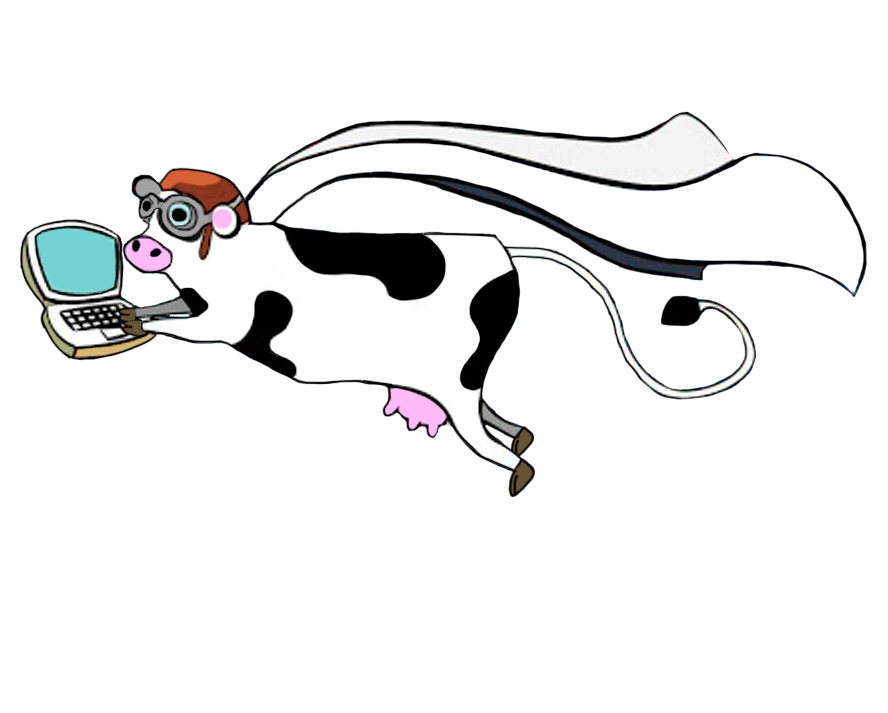
\includegraphics[scale=.2]{../imagenes/logoo.png}
\end{center}
\subsection*{Slogan}
\begin{center}
  \textit{``¿En qué término prefiere su software?''}
                          
\end{center}

\rule{0.8\textwidth}{.8pt}\\

\subsection*{Misión}
Brindar servicios de software de buena calidad, analizando los riesgos que
podrían afectar a nuestros clientes.

\rule{0.8\textwidth}{.8pt}\\

\subsection*{Visión}
Apoyar, creer y motivar a cualquiera en el mercado que necesite de la tecnología.

\rule{0.8\textwidth}{.8pt}\\

\subsection*{Valores}

\begin{itemize}
\item Transparencia.
\item Puntualidad.
\item Responsabilidad
\item Pasión.
\item Resolución.
\end{itemize}

\rule{0.8\textwidth}{.8pt}\\

\subsection*{Involucrados}
\subsubsection*{Equipo de trabajo}
\begin{itemize}
\item Galeana Araujo Emiliano. 314032324 Responsable Técnico.
\item Jardines Mendoza César Eduardo. 314071549 Responsable de Calidad.
\item Mendoza Castillo María Fernanda. 314280587 Líder de equipo.
\end{itemize}

\subsubsection*{Docentes}
\begin{itemize}
\item Profesor: Selene Marisol Martínez Ramírez
\item Ayudante: Arturo Castillo Valles
\item Ayud. Laboratorio: Luis Rey Rutiaga Robles
\end{itemize}

\rule{0.8\textwidth}{.8pt}\\

\newpage
\section*{Producto de Software}

\subsection*{Nombre del producto de software}
CafeCiencias\\

\rule{0.8\textwidth}{.8pt}\\

\subsection*{Metodología}
\subsubsection*{Desarrollo de Software}
\begin{itemize}
\item SCRUM
\item Kanban
\end{itemize}
\subsubsection*{Manejo de Riesgos}
\begin{itemize}
\item FODA
\item Diagrama de Tortuga
\end{itemize}

\rule{0.8\textwidth}{.8pt}\\

\subsection*{Periodo}
Fecha de inicio: 20 de Marzo de 2020\\
\indent Fecha de fin: 9 de Mayo de 2020\\


\rule{0.8\textwidth}{.8pt}\\

\subsection*{Repositorio común de documentos}
\href{https://sites.google.com/view/vakas-lokas/p\%C3\%A1gina-principal?authuser=1}{Página de la empresa}

\href{https://drive.google.com/open?id=13f9jp3Oli6AQF1Ap8VhoEKFXTPULumos}{RT-2020-Drive}

\href{https://github.com/mildewyPrawn/CafeCiencias}{RT-2020-Repositorio}

\href{https://trello.com/b/rwdAGuSi/cafeciencias}{RT-2020-Trello}

\rule{0.8\textwidth}{.8pt}\\

\subsection*{Propuesta de Proyecto Final}

“CafeCiencias” será una aplicación web destinada a las personas que suelen o
deseen ir a comer a la cafetería de la Facultad de Ciencias, así como el personal
de la cafetería. Esta aplicación ofrecerá una manera mas práctica y fácil de
saber los horarios, el menú de la comidas, sus precios, avisos y si alguna de las
comidas ya se  acabó. Además los usuarios podrán informar a otros sobre retrasos
en los horarios o la entrega de algunos platillos.

\rule{0.8\textwidth}{.8pt}\\

\subsection*{Casos de uso}

\begin{center}
  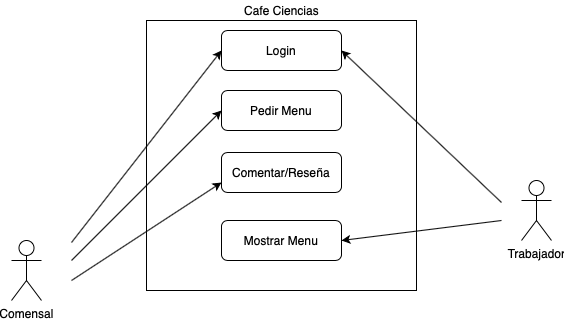
\includegraphics[scale=.75]{../imagenes/CasoDeUsos.png}
\end{center}

\rule{0.8\textwidth}{.8pt}\\

\subsection*{Propuesta de Valor}

La aplicación ofrece un acercamiento al momento entre la cafetería de la
Facultad con los clientes pues además de revisar al día los menús y precios,
habrá una discusión entre los mismos clientes para garantizar notificaciones
comunitarias en tiempo real evitando tener que ir a la cafetería.

\rule{0.8\textwidth}{.8pt}\\

\subsection*{Tipos de Usuarios}

La aplicación va dirigida en su mayoría a estudiantes, trabajadores y profesores
de la Facultad de Ciencias que disfruten de comer en la cafetería principal.
Aunque también pueden hacer uso de esta, personas que laboren en otra facultad,
instituto, dependencia de la UNAM. Y en casos extremos, personas ajenas a la
Universidad que gusten de comer ahí. 

El otro tipo de usuarios son trabajadores de la cafetería principal de la
facultad de ciencias, siendo ellos quienes actualizan el menú.

\rule{0.8\textwidth}{.8pt}\\

\subsection*{Tecnologías para la Implementación}

\begin{center}
  \begin{tabular}{| c | c | c | c | } \hline
    Concepto & Herramienta & Versión & Función \\\hline
    Framework & django & 2.2.4 & Para complementar funciones del lenguaje python. \\\hline
    Diagramador UML & draw.io & 11.2.8 &  Para realizar los diagramas \\\hline
    Manejador de bases de datos & sqlite3 & 3.31.1 & Para almacenar las bases de
    datos y operar con ellas. \\\hline
    IDE & Sublime & 3 & Para escribir \\
    & Emacs & 26.3 & código \\\hline
    Control de versiones & git & 2.23.0 & Para controlar las versiones y tener y \\
    & & & apoyarnos la producción del producto. \\ \hline
  \end{tabular}
\end{center}

\rule{0.8\textwidth}{.8pt}\\

\end{document}
